% !TEX program = xelatex
\documentclass[UTF8,a4paper,12pt]{ctexart}
\usepackage{geometry}
\geometry{left=2.5cm,right=2.5cm,top=2.5cm,bottom=2.5cm}
\usepackage{amsmath,amssymb,bm}
\usepackage{graphicx}
\usepackage{booktabs,array,multirow}
\usepackage{subcaption}
\usepackage{enumitem}
\usepackage{float}
\usepackage{hyperref}
\hypersetup{hidelinks}
\graphicspath{{exp1_images/}}
\newcommand{\blank}[1][2.5cm]{\mbox{\underline{\hspace{#1}}}}
\newcommand{\answer}{\par\noindent\textbf{填写：}\blank[0.86\textwidth]\par}
\numberwithin{equation}{section}

\title{《一维冲击应力波的测量》实验报告}
\author{姓名\blank[2.5cm] \quad 学号\blank[3cm] \quad 同组成员\blank[4cm]\\[1em]
实验地点\blank[3cm] \quad 实验日期\blank[4cm]}
\date{}
\begin{document}
\maketitle
\tableofcontents
\clearpage

\section{实验目的}
\begin{enumerate}
  \item 掌握测量一维冲击应力波的原理和方法。
  \item 学会超动态应变仪和数字存储示波器的操作、使用。
  \item 测量金属材料（40铬钢和 LY12CZ 铝）的一维纵波波速和动态弹性模量。
  \item 测量应力波在不同材料界面上传播时的透射率和反射率，并验证在不同材料界面上传播的一维应力波理论。
  \item 分析测试结果，探讨材料静动态性能的差别、一维纵波的传播特性及一维纵波理论的适用性。
  \item 分析测量误差，并讨论提高精度的方法。
\end{enumerate}

\section{实验装置、仪器及器材}
\begin{enumerate}
  \item 一维冲击压杆实验装置（北大自研；支撑杆件、保证与空气枪的链接、阻挡杆件飞出）。
  \item KDQ-1 空气动力枪（兵器工业部二〇八所制造）。
  \item SDY2107 超动态应变仪（北戴河实用电子技术研究所）、SDY2301 应变仪桥盒（北戴河实用电子技术研究所）。
  \item 数字存储示波器（Tektronix TDS2024 FOUR CHANNEL DIGITAL STORAGE OSCILLOSCOPE，200 MHz，2 GS/s）。
  \item 贴好应变片的铝杆和钢杆若干。
  \item 天平（BSM3200.2 电子天平，上海卓精电子科技有限公司，最大量程 3200 g，最小称量 0.2 g）、碳钢游标卡尺（福吉斯特工具，7D-01150，0--150 mm，50 分度）、直尺（广塑十四厂，0--50 cm，1 mm 分度）。
  \item 加载头、子弹、镊子。
\end{enumerate}

\section{实验测量方法与测量过程}
\subsection{一维纵波实验测材料动态力学性能的方法}
本实验基于 Hopkinson 压杆实验装置，直接测试压杆的一维应力波传播特性，具体的实验装置及测量系统如图\ref{fig:exp1-system}所示。Hopkinson 压杆实验由两部分组成：第一部分测定钢、铝两种材料的波速、密度及动态弹性模量；第二部分测定钢、铝两种材料的透射系数、反射系数。

为了保证一维应力波理论成立，所有圆柱形压杆的横截面尺寸都相同。加载头的作用是为了防止子弹直接打到输入杆上，把杆端面打坏（不平整）或不是打在杆端面的中心。这里采用超动态应变仪和数字存储示波器进行动态应变资料的采集与记录。由于冲击过程中应变变化剧烈，可近似看作绝热过程。因此，本实验不需要温度补偿，每个应变片采用四分之一电桥测试。具体两部分测量方法如下所示。

\begin{figure}[H]
  \centering
  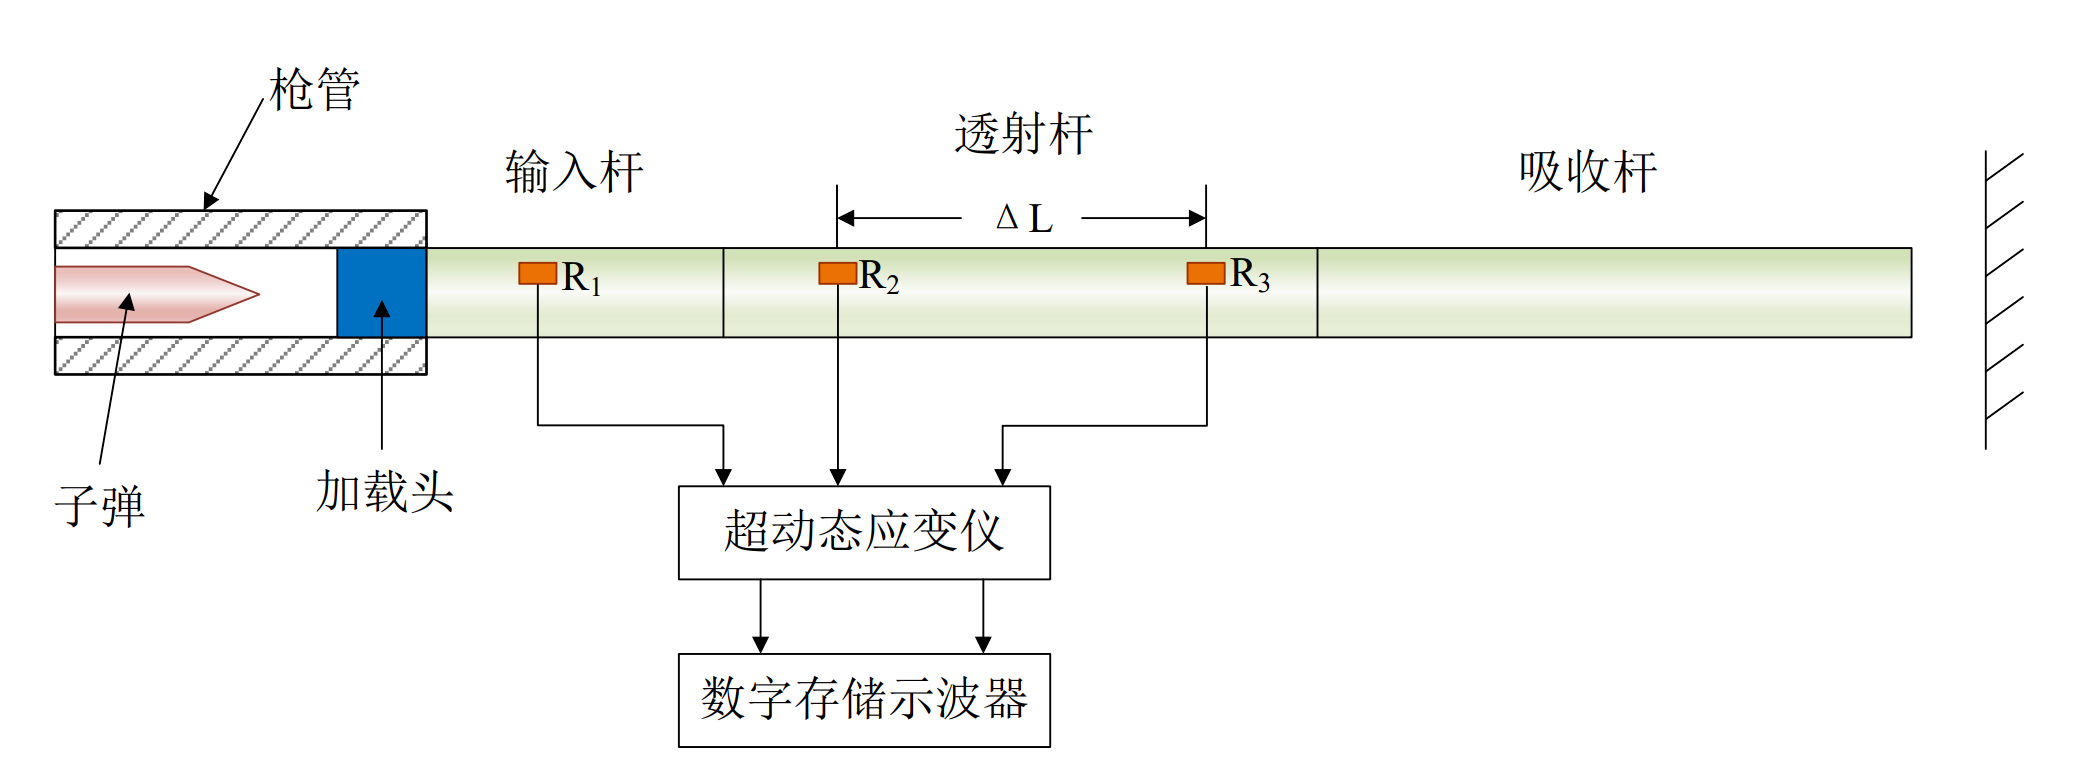
\includegraphics[width=0.72\textwidth]{p03_img01.png}
  \caption{实验装置及测量系统示意图}
  \label{fig:exp1-system}
\end{figure}

\subsubsection{一维纵波波速及动态弹性模量的测定}
当枪膛内子弹以某一速度撞击加载头时，加载头将把这一应力脉冲传输给输入杆，并在杆中产生入射脉冲 $\varepsilon_i(t)$。其中输入杆、透射杆和吸收杆都采用材料、截面尺寸相同的压杆，通过测量透射杆上 $R_2$ 和 $R_3$ 两个应变片的动态应变随时间变化曲线，得到应力波到达这两个应变片的时间差，便可以得到应变波从 $R_2$ 传播到 $R_3$ 所需要的时间 $\Delta T$。这样根据两个应变片相隔的距离 $\Delta L$，可以得到一维纵波在该材料中传播的速度
\begin{equation}
  C_0=\frac{\Delta L}{\Delta T}.
  \label{eq:exp1-speed}
\end{equation}
由一维应力波理论可测得该材料的动态弹性模量为
\begin{equation}
  E_d=C_0^2\rho,
  \label{eq:exp1-modulus}
\end{equation}
其中 $\rho$ 为材料的密度。

\subsubsection{一维纵波在不同材料界面中的传播}
为了测定一维纵波在不同材料接口中传播时应力波的透射系数 $n_t$ 和反射系数 $n_r$，透射杆和吸收杆都选用与入射杆不同材料的杆，其中透射杆后面的吸收杆需选用与其材料、截面相同的杆，以避免界面反射的脉冲波影响应变测量结果。输入杆中的入射脉冲 $\varepsilon_i(t)$ 沿杆传播到与透射杆相连的界面，会产生往回传播的反射脉冲 $\varepsilon_r(t)$ 和向前传播的透射脉冲 $\varepsilon_t(t)$。

通过测量输入杆和透射杆上的应变片 $R_1$ 和 $R_2$ 的动态应变，再根据标定值，可得 $\varepsilon_i(t)$ 和 $\varepsilon_r(t)$。由一维胡克定律 $\sigma=E_d\varepsilon$，可以计算出相应的应力 $\sigma_i(t)$ 和 $\sigma_t(t)$。由在输入杆和透射杆界面上的应力连续条件，可得
\begin{equation}
  \sigma_i+\sigma_r=\sigma_t.
\end{equation}
因此，由 $\varepsilon_i(t)$ 和 $\varepsilon_r(t)$ 最大幅值点计算出 $\sigma_i$ 和 $\sigma_t$ 后，由一维纵波理论有
\begin{subequations}
\begin{align}
  n_r&=\frac{\sigma_r}{\sigma_i}
      =\frac{\rho_2C_2-\rho_1C_1}{\rho_1C_1+\rho_2C_2},\\
  n_t&=\frac{\sigma_t}{\sigma_i}
      =\frac{2\rho_2C_2}{\rho_1C_1+\rho_2C_2}.
\end{align}
\end{subequations}
式中 $\rho_1$ 和 $C_1$ 分别是输入杆的材料密度和波速，$\rho_2$ 和 $C_2$ 分别是透射杆的材料密度和波速。

\subsection{实验测量过程}
本实验大致分三步进行：第一步是 Hopkinson 压杆的安装和空气动力枪的准备工作；第二步是超动态应变仪和数字存储示波器的调试、准备工作；第三步是用空气动力枪射弹，同时由超动态应变仪和数字存储示波器采集。

\subsubsection{Hopkinson 压杆实验装置的准备工作}
\begin{enumerate}
  \item 实验要求：Hopkinson 压杆实验的数据处理是建立在一维假定基础上的，所以在这里应尽量保证一维应力波理论仍然成立。
  \item Hopkinson 压杆安装：根据实验要求选择合适的输入杆、透射杆和吸收杆。安装时要仔细调节导轨上的螺钉，使三根杆及加载头之间每个界面都要完全接触（不能有缝隙），界面完全重合（不能错开），且保证杆轴都在同一条直线上。
\end{enumerate}

\subsubsection{空气动力枪的操作}
\begin{enumerate}
  \item 接通电源后，打开电源开关（红灯显示）。
  \item 装弹：一手将枪机手柄向后拉到位，另一只手用镊子将子弹装入枪膛（注意弹头方向）后，松开手柄。
  \item 供气：打开高压气瓶阀门，轻轻向左旋转进气阀手轮（左边的手轮），压力表指针移动，同时旋转调压阀手轮使指针略高于所需压力标度，关上进气阀，再微调调压阀手轮使指针稳定在所需压力标度。
  \item 供弹：按“供弹”开关，用压缩空气推动枪机，将子弹推到位。
  \item 射击：按动射击开关（绿灯显示），子弹出射。
  \item 工作结束后的操作：关上高压气瓶阀门。按动供弹开关，启动供弹电磁阀，直到将余气放净。如电源已断，可手动电磁阀上的手动开关放气。最后，断开电源。
\end{enumerate}

\subsubsection{仪器调试}
\begin{enumerate}
  \item 接通超动态应变仪和瞬态波形存储器的电源。
  \item 将应变片的测量导线分别接到应变仪的对应信道的输入端上。超动态应变仪采用惠斯通电桥式电路。由于冲击载荷的作用时间极短（通常几十微秒的量级），即使考虑到应力波的传播、反射等过程，一般也就几百微秒，这么短的时间也不必考虑温度补偿。因此，选择 $1/4$ 桥路进行应变测量。
  \item 将应变仪各个测量信道的输出端与数字存储示波器对应信道的输入端接通。
  \item 标定：应在测试开始前，对超动态应变仪各个通道进行标定。进入标定模式，估计被测应变的幅值大小，适当选择应变仪的标定档。应当注意的是，标定好后，超动态应变仪和数字存储示波器的衰减旋钮和开关都不能再动。
\end{enumerate}

\subsubsection{测试步骤}
本实验中分别做以下四种情况的实验：
\begin{enumerate}[label=\alph*)]
  \item 输入杆、透射杆和吸收杆全部是铝杆，测波速 $C_{al}$。
  \item 上述三根杆全部换成钢杆，测波速 $C_{st}$。
  \item 输入杆用铝杆，透射杆和吸收杆是钢杆，测 $\varepsilon_i(t)$ 和 $\varepsilon_t(t)$。
  \item 与上一种情况相反，输入杆用钢杆，透射杆和吸收杆用铝杆，也测 $\varepsilon_i(t)$ 和 $\varepsilon_t(t)$。
\end{enumerate}
以上四个实验分别按以下步骤进行：
\begin{enumerate}
  \item 将输入杆、透射杆和吸收杆安装好，并调好空气动力枪的气压，将子弹供弹到位。
  \item 选择合适的“采样速度”。
  \item 选好触发方式。采用内触发，应选先到的信号作为触发，并将信道开关指向该信道，再调好触发电平。
  \item 使“写等待”指示灯亮，这时全部准备工作即告完成。试验时，按空气动力枪的“射击”开关，数字存储示波器即按所规定的“采样速度”将超动态应变仪上的信号一个个采样，并存入内存中。如果需要，可通过数字存储示波器的专用接口与计算机连接，将记录的资料送入计算机进行分析处理后再将结果打印或绘图。
  \item 用没有贴应变片的铝杆和钢杆，量一下几何尺寸及质量，测出密度 $\rho_{al}$ 和 $\rho_{st}$。
\end{enumerate}

\section{铝和钢的波速及动态弹性模量}
\subsection{材料密度测量}
分别多次测量材料质量 $m$ 和几何参数，将本组测量结果记入表\ref{tab:exp1-density}。

\begin{table}[H]
\centering
\caption{试件质量和尺寸测量结果}
\label{tab:exp1-density}
\begin{tabular}{llcccc}
\toprule
\multicolumn{2}{l}{测量对象} & 测量1 & 测量2 & 测量3 & 均值\\
\midrule
\multirow{3}{*}{钢} & 质量（g） & \blank[1.3cm] & \blank[1.3cm] & \blank[1.3cm] & \blank[1.3cm]\\
 & 直径（mm） & \blank[1.3cm] & \blank[1.3cm] & \blank[1.3cm] & \blank[1.3cm]\\
 & 长度（mm） & \blank[1.3cm] & \blank[1.3cm] & \blank[1.3cm] & \blank[1.3cm]\\
\midrule
\multirow{3}{*}{铝} & 质量（g） & \blank[1.3cm] & \blank[1.3cm] & \blank[1.3cm] & \blank[1.3cm]\\
 & 直径（mm） & \blank[1.3cm] & \blank[1.3cm] & \blank[1.3cm] & \blank[1.3cm]\\
 & 长度（mm） & \blank[1.3cm] & \blank[1.3cm] & \blank[1.3cm] & \blank[1.3cm]\\
\bottomrule
\end{tabular}
\end{table}

由此可以计算得，钢的密度测量结果为
\begin{equation}
  \bar{\rho}_{st}=\frac{4\bar{m}_{st}}{\pi\bar{d}_{st}^{\,2}\bar{l}_{st}}
  =\blank[2cm]\ \mathrm{g/cm^3}.
\end{equation}
同理，铝的密度测量结果为
\begin{equation}
  \bar{\rho}_{al}=\frac{4\bar{m}_{al}}{\pi\bar{d}_{al}^{\,2}\bar{l}_{al}}
  =\blank[2cm]\ \mathrm{g/cm^3}.
\end{equation}

\subsection{应变仪标定}
超动态应变仪能够将应变信号转化为电压信号，但是我们并不知道多大的应变对应多大的电压，故需要进行标定操作。这里采用负校，通过施加多种应变测得对应应力值，并取平均，计算得到单位电压对应的应变。两个通道中给定应变与输出电压关系如表\ref{tab:exp1-calibration}所示。

\begin{table}[H]
\centering
\caption{应变仪标定中给定应变与输出电压关系}
\label{tab:exp1-calibration}
\begin{tabular}{lcccc}
\toprule
标定对象 & $30\times100\,\mu\varepsilon$ & $40\times100\,\mu\varepsilon$ & $50\times100\,\mu\varepsilon$ & 单位电压对应的应变\\
\midrule
通道1 & \blank[1.5cm] & \blank[1.5cm] & \blank[1.5cm] & \blank[2cm]\\
通道2 & \blank[1.5cm] & \blank[1.5cm] & \blank[1.5cm] & \blank[2cm]\\
\bottomrule
\end{tabular}
\end{table}

\subsection{测量波速}
因为撞击是一个瞬态过程，无法通过手动方式控制示波器是否开始录入数据，因此使用内触发并设置触发电平。记录本组实验参数：当入射杆为钢时，触发电平为\blank[2cm]，空气动力枪气压为\blank[2cm]；当入射杆为铝时，触发电平为\blank[2cm]，空气动力枪气压为\blank[2cm]；采样频率为\blank[2cm]。测量数据如表\ref{tab:exp1-distance}和表\ref{tab:exp1-time}所示。

\begin{table}[H]
\centering
\caption{两根入射杆中两个应变片的距离}
\label{tab:exp1-distance}
\begin{tabular}{lcccc}
\toprule
测量对象 & 测量1 & 测量2 & 测量3 & 均值\\
\midrule
钢（cm） & \blank[1.5cm] & \blank[1.5cm] & \blank[1.5cm] & \blank[1.5cm]\\
铝（cm） & \blank[1.5cm] & \blank[1.5cm] & \blank[1.5cm] & \blank[1.5cm]\\
\bottomrule
\end{tabular}
\end{table}

\begin{table}[H]
\centering
\caption{两根入射杆中应变波的时间差}
\label{tab:exp1-time}
\begin{tabular}{lccc}
\toprule
测量对象 & 波前时间差 & 波峰时间差 & 均值\\
\midrule
钢（$\mu$s） & \blank[1.8cm] & \blank[1.8cm] & \blank[1.8cm]\\
铝（$\mu$s） & \blank[1.8cm] & \blank[1.8cm] & \blank[1.8cm]\\
\bottomrule
\end{tabular}
\end{table}

根据公式\eqref{eq:exp1-speed}，计算可得
\begin{subequations}
\begin{align}
  C_{st}&=\blank[2.5cm]\ \mathrm{m/s},\\
  C_{al}&=\blank[2.5cm]\ \mathrm{m/s}.
\end{align}
\end{subequations}

\subsection{动态弹性模量测量}
已知材料的波速和密度，由公式\eqref{eq:exp1-modulus}计算材料的动态弹性模量：
\begin{subequations}
\begin{align}
  E_{d,st}&=C_{st}^2\rho_{st}=\blank[2.5cm]\ \mathrm{GPa},\\
  E_{d,al}&=C_{al}^2\rho_{al}=\blank[2.5cm]\ \mathrm{GPa}.
\end{align}
\end{subequations}

\section{反射、透射系数测量}
\subsection{实验计算结果}
入射杆为钢杆、透射杆和吸收杆为铝杆时，触发电平为\blank[2cm]，空气动力枪气压为\blank[2cm]；入射杆为铝杆、透射杆和吸收杆为钢杆时，触发电平为\blank[2cm]，空气动力枪气压为\blank[2cm]。空气动力枪发射后，将记录数据填入表\ref{tab:exp1-amplitude}，并计算透射系数和反射系数。

\begin{table}[H]
\centering
\caption{两个入射杆中应变波的峰谷幅值}
\label{tab:exp1-amplitude}
\begin{tabular}{lcc}
\toprule
测量对象 & 钢$\rightarrow$铝 & 铝$\rightarrow$钢\\
\midrule
通道一第一次波峰谷幅值（V） & \blank[2cm] & \blank[2cm]\\
通道二第一次波峰谷幅值（V） & \blank[2cm] & \blank[2cm]\\
\bottomrule
\end{tabular}
\end{table}

\subsubsection{钢\texorpdfstring{$\rightarrow$}{→}铝}
入射杆和透射杆的应变分别为
\begin{subequations}
\begin{align}
  \varepsilon_i&=\blank[1.2cm]\times\blank[1.2cm]\times10^{-6}=\blank[1.8cm],\\
  \varepsilon_t&=\blank[1.2cm]\times\blank[1.2cm]\times10^{-6}=\blank[1.8cm].
\end{align}
\end{subequations}
入射杆和透射杆的应力分别为
\begin{subequations}
\begin{align}
  \sigma_i&=E_{d,st}\varepsilon_i=\blank[2cm]\ \mathrm{MPa},\\
  \sigma_t&=E_{d,al}\varepsilon_t=\blank[2cm]\ \mathrm{MPa}.
\end{align}
\end{subequations}
透射系数与反射系数分别为
\begin{subequations}
\begin{align}
  n_t&=\frac{\sigma_t}{\sigma_i}=\blank[2cm],\\
  n_r&=\frac{\sigma_t}{\sigma_i}-1=\blank[2cm].
\end{align}
\end{subequations}

\subsubsection{铝\texorpdfstring{$\rightarrow$}{→}钢}
入射杆和透射杆的应变分别为
\begin{subequations}
\begin{align}
  \varepsilon_i&=\blank[1.2cm]\times\blank[1.2cm]\times10^{-6}=\blank[1.8cm],\\
  \varepsilon_t&=\blank[1.2cm]\times\blank[1.2cm]\times10^{-6}=\blank[1.8cm].
\end{align}
\end{subequations}
入射杆和透射杆的应力分别为
\begin{subequations}
\begin{align}
  \sigma_i&=E_{d,al}\varepsilon_i=\blank[2cm]\ \mathrm{MPa},\\
  \sigma_t&=E_{d,st}\varepsilon_t=\blank[2cm]\ \mathrm{MPa}.
\end{align}
\end{subequations}
透射系数与反射系数分别为
\begin{subequations}
\begin{align}
  n_t&=\frac{\sigma_t}{\sigma_i}=\blank[2cm],\\
  n_r&=\frac{\sigma_t}{\sigma_i}-1=\blank[2cm].
\end{align}
\end{subequations}

\subsection{一维纵波理论计算结果}
根据一维纵波理论，通过材料密度和波速计算透射系数和反射系数。

\subsubsection{钢\texorpdfstring{$\rightarrow$}{→}铝}
\begin{subequations}
\begin{align}
  n_t&=\frac{2\rho_{al}C_{al}}{\rho_{st}C_{st}+\rho_{al}C_{al}}=\blank[2cm],\\
  n_r&=\frac{\rho_{al}C_{al}-\rho_{st}C_{st}}{\rho_{st}C_{st}+\rho_{al}C_{al}}=\blank[2cm].
\end{align}
\end{subequations}

\subsubsection{铝\texorpdfstring{$\rightarrow$}{→}钢}
\begin{subequations}
\begin{align}
  n_t&=\frac{2\rho_{st}C_{st}}{\rho_{al}C_{al}+\rho_{st}C_{st}}=\blank[2cm],\\
  n_r&=\frac{\rho_{st}C_{st}-\rho_{al}C_{al}}{\rho_{al}C_{al}+\rho_{st}C_{st}}=\blank[2cm].
\end{align}
\end{subequations}

\section{结果分析与讨论}
将本组一维应力波波速汇总于表\ref{tab:exp1-speed-summary}，并比较钢和铝的测量结果。

\begin{table}[H]
\centering
\caption{钢和铝中一维应力波波速}
\label{tab:exp1-speed-summary}
\begin{tabular}{lcc}
\toprule
测量对象 & 钢 & 铝\\
\midrule
一维应力波波速（m/s） & \blank[2.5cm] & \blank[2.5cm]\\
\bottomrule
\end{tabular}
\end{table}
\answer

根据应力波波速与密度计算材料的弹性模量，并与静态弹性模量比较，结果填入表\ref{tab:exp1-modulus-summary}。

\begin{table}[H]
\centering
\caption{钢和铝的弹性模量}
\label{tab:exp1-modulus-summary}
\begin{tabular}{lcc}
\toprule
测量对象 & 实验测得动态弹性模量 & 静态弹性模量\\
\midrule
钢（GPa） & \blank[2.5cm] & 210\\
铝（GPa） & \blank[2.5cm] & 68\\
\bottomrule
\end{tabular}
\end{table}

在高应变率实验时，必须充分考虑试件的惯性效应。当试件经历应变时，由于分子重排所需的时间，所产生的应力与应变之间存在相位差。通过相位分析可以得知，应力可分为两部分：一部分与应变同相位，另一部分与应变相位差为 $90$ 度。因此，在高应变率条件下，弹性模量由两部分组成：一部分是应力与同相位应变之比（即静态弹性模量），另一部分则是应力与不同相位应变之比。结合本组结果分析动态弹性模量与静态弹性模量的差异及可能原因。
\answer

不同材料界面上的透射系数与反射系数汇总于表\ref{tab:exp1-coefficient-summary}。

\begin{table}[H]
\centering
\caption{透射系数与反射系数计算结果}
\label{tab:exp1-coefficient-summary}
\begin{tabular}{llcc}
\toprule
\multicolumn{2}{l}{测量对象} & 透射系数 & 反射系数\\
\midrule
\multirow{3}{*}{钢$\rightarrow$铝} & 实验结果 & \blank[1.8cm] & \blank[1.8cm]\\
 & 一维纵波理论结果 & \blank[1.8cm] & \blank[1.8cm]\\
 & 相对误差 & \blank[1.8cm] & \blank[1.8cm]\\
\midrule
\multirow{3}{*}{铝$\rightarrow$钢} & 实验结果 & \blank[1.8cm] & \blank[1.8cm]\\
 & 一维纵波理论结果 & \blank[1.8cm] & \blank[1.8cm]\\
 & 相对误差 & \blank[1.8cm] & \blank[1.8cm]\\
\bottomrule
\end{tabular}
\end{table}

由密度和波速求透射系数和反射系数的实验原理是一维纵波理论。分析实验结果能否验证一维纵波理论，并讨论实际测量值与理论计算值出现偏差的原因。
\answer

误差的可能来源及改进方法如下，请结合本组实际情况补充和修改：
\begin{enumerate}
  \item Hopkinson 压杆实验仪器使用年限较长，实验杆件截面可能发生变形，且很难保证截面完全对齐，会产生一定的能量损失。若杆与杆的接触面无法完全接触，被传递应力的杆可能产生偏心压缩，进而产生弯曲波，从而无法保证一维应力波假设。
  \item 入射杆、透射杆和吸收杆在安装时存在误差。由于控制水平的方式是通过拧两个螺丝完成，很难确保三杆轴线处在同一直线上，这也会影响一维应力波假设。
  \item 入射杆、透射杆和吸收杆在仪器上的运动可能受到滚动钢珠的约束，在接触点中产生摩擦力，从而出现新的波源干扰实验。
  \item 读数误差：不同通道的电压值是通过波谷与电压平衡时的差值读出的，这一过程可能存在误差。测量两个应变片之间的距离时会受到已粘贴应变片的约束；测量钢和铝的密度时分别使用其中一根杆件计算，也很难保证同种材质的全部杆件密度都等于该测量值。
  \item 由实验求透射系数和反射系数，需要先把电压转化为应变，再把应变转化为应力，最后由应力求比值得到结果。这个计算过程涉及的物理量都是状态量，不同大小的外部输入会得到不同大小的状态量，因此计算结果受实验开始前仪器参数的影响较大。
  \item 根据一维应力波理论计算透射系数和反射系数时，所需波速根据透射杆应变测得，密度根据材料试件测得；而实验测得的透射和反射系数由入射杆和透射杆数据得到，这也可能导致误差。
  \item 温度、湿度等外部条件会对实验环境产生一定影响。虽然冲击过程可近似视为绝热，但设备与环境温度的微小差异仍可能导致误差。
  \item 当输入杆为铝杆、透射杆和吸收杆为钢杆时，若误差较大，可考虑巨大冲击是否给输入铝杆造成损伤或塑性变形。
\end{enumerate}

注意观察杆碰撞后各通道在第一个波谷之后是否出现第二个波峰，并分析其是否由应力波到达铝和钢的边界后发生反射所产生。若将这部分考虑进去，可能有助于更好地计算反射系数。
\answer

可通过增加辅助设备确保杆架平行；在杆件和滚动钢珠之间适当润滑，减少摩擦对实验的影响；完整测量材料密度；准确刻画应变片之间的距离；在时间允许的情况下增加实验次数，多次测量取平均值。结合本组情况写出其他提高精度的方法。
\answer

\end{document}
